%\section{Gaussmeter LabView Protocol}
\label{app:LabView}

Figure~\ref{fig:gaussmeter-flowchart}. Upon startup, the \gls{lvi} initializes serial communication with the Gaussmeter, loads user-defined parameters (such as file name, mode of acquisition, delay time, and probe coordinates), and clears buffers in preparation for logging. The user may select either a continuous or an individual sampling mode. In continuous mode, the \gls{lvi} iterates through a defined number of data points with a fixed delay between samples; in individual mode, each data capture is triggered manually, allowing for precise positioning or timing. For both modes, each cycle involves reading the spatial coordinates, sending a measurement command, recording the returned magnetic flux value, and updating a graphical display as well as the output file.

While the flowchart reflects the core logic, it does not fully convey the customization added to the \gls{lvi} interface. For example, the front panel includes input fields for patient table (couch) parameters such as couch speed and displacement points. As mentioned above, phantom is discretized with radial and angular indices: angular positions span 12 sectors clockwise from the 12 o’clock position (0 to 11 or A to L), and radial depths range from the center (0) to the outer edge (6). The probe’s spatial location is represented in polar coordinates, and the system plots magnetic flux as a function of position rather than time, allowing for intuitive visualization of the MRI fringe field across the phantom surface.
The \gls{lvi} is operated in the following way.

Flowchart of the Gaussmeter VI data acquisition algorithm
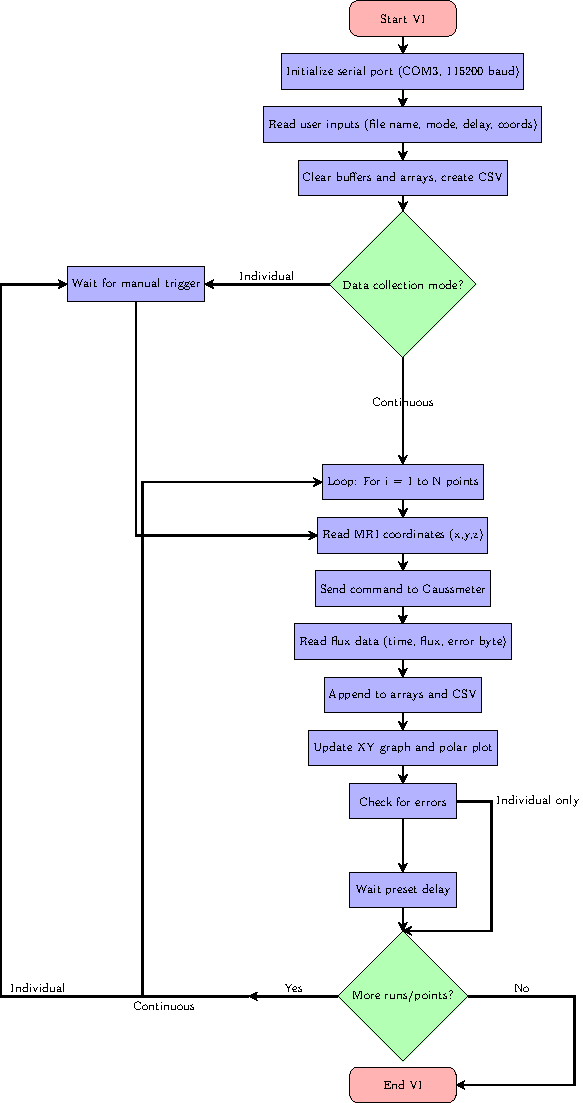
\includepdf[
pages=1,
landscape=false,
scale=0.90,
]{TikZ/flowchart.pdf}
\label{fig:gaussmeter-flowchart}

\section{Sample Data for Stray Magnetic Field Mapping Along the Patient Couch (Backward Pass at (0,0))}
\label{app:DataStrayField}

As mentioned in Section \ref{sec:metClinic_flux}, Table \ref{tab:sampleStrayFieldBackward} presents a representative subset of the raw dataset from the first backward (retracting) couch translation pass along the longitudinal (z) axis at the central grid coordinate (0,0). Data were logged continuously using the Hall-effect gaussmeter probe. Flux values are raw instrument readings in gauss. The err\_byte column is the gaussmeter's reported error code.

Uncertainties: position $\pm 1$ mm (couch display and alignment tolerance), time $\pm 0.01$ s, flux $\pm 0.2\%$ of reading or $\approx \pm 50$ G near full scale.

\begin{table}[htbp]
	\centering
	\footnotesize
	\begin{tabular}{c c c c c c}
		\hline
		z$_{\text{pos}}$ [mm] & x$_{\text{pos}}$ [mm] & y$_{\text{pos}}$ [mm] & time [s] & flux [G] & err\_byte \\
		\hline
		0  & 0 & 0 & 0.25  & 26823 & 64.039 \\
		0  & 0 & 0 & 0.50  & 26823 & 64.289 \\
		0  & 0 & 0 & 1.00  & 26822 & 64.788 \\
		0  & 0 & 0 & 2.00  & 26824 & 65.788 \\
%		0  & 0 & 0 & 2.75  & 26672 & 66.539 \\
		0  & 0 & 0 & 3.50  & 24245 & 67.290 \\
%		0  & 0 & 0 & 4.00  & 22911 & 67.790 \\
		0  & 0 & 0 & 5.00  & 20287 & 68.791 \\
%		0  & 0 & 0 & 6.00  & 16493 & 69.789 \\
		0  & 0 & 0 & 7.00  & 14331 & 70.788 \\
%		0  & 0 & 0 & 10.00 & 8534  & 73.796 \\
		0  & 0 & 0 & 12.00 & 5886  & 75.803 \\
		0  & 0 & 0 & 15.00 & 3563  & 78.807 \\
%		0  & 0 & 0 & 17.00 & 2529  & 80.804 \\
		0  & 0 & 0 & 20.00 & 1607  & 83.805 \\
%		0  & 0 & 0 & 23.00 & 1053  & 86.800 \\
		0  & 0 & 0 & 25.00 & 794   & 88.798 \\
%		0  & 0 & 0 & 27.00 & 640   & 90.800 \\
%		0  & 0 & 0 & 29.00 & 570   & 92.801 \\
		0  & 0 & 0 & 30.00 & 570   & 93.801 \\
		\hline
	\end{tabular}
	\caption[Representative raw data – backward pass at (0,0)]{Subset of measurements from the first retracting translation along the z-axis at isocenter (grid 00). Flux decreases as the probe moves away from the bore entrance. Full dataset (120 rows) and all 15 CSV files were imported into Python with pandas for cleaning, alignment of forward/backward pairs, and numerical computation of the longitudinal gradient $\partial B / \partial z$.}
	\label{tab:sampleStrayFieldBackward}
\end{table}

\section{Sample Data for Translational Force Experiment}
\label{app:DataTrans}

Table \ref{tab:sampleData} presents a representative subset of the displacement–current dataset used for field–gradient and angle calculations for experiment en section \ref{sec:experiment1}
Uncertainties: position $\pm 0.05$ mm, current $\pm 0.001$ A.

\begin{table}[h!]
	\centering
	\footnotesize
	\begin{tabular}{c c c c c c c c c}
		\hline
		N & $x$ [mm] & $I$ [A] & $B_{-0.5}$ & $B_0$ & $B_{+0.5}$ & $dB/dx$ & $\theta$ & $B_0\,dB/dx$  \\
		\hline
		1  & 0  & 0.000 & --    & --    & --    & --          & --            & -- \\
		2  & 1  & 0.554 & 2.86  & 2.81  & 2.84  & 0.1111      & 0.001047      & 0.3123 \\
		3  & 2  & 1.221 & 5.56  & 5.66  & 5.70  & 1.4444      & 0.002094      & 8.1691 \\
		4  & 3  & 1.636 & 7.03  & 7.22  & 7.24  & 2.1111      & 0.003141      & 15.2469 \\
		5  & 4  & 2.217 & 9.32  & 9.44  & 9.44  & 1.2222      & 0.004188      & 11.5432 \\
		6  & 5  & 2.471 & 10.27 & 10.40 & 10.56 & 2.8889      & 0.005235      & 30.0444 \\
		7  & 6  & 2.752 & 11.61 & 11.66 & 11.80 & 1.8889      & 0.006282      & 22.0160 \\
		8  & 7  & 2.966 & 12.58 & 12.63 & 12.76 & 1.7778      & 0.007329      & 22.4593 \\
		9  & 8  & 3.196 & 13.92 & 14.02 & 14.27 & 3.4444      & 0.008377      & 48.2988 \\
		10 & 9  & 3.507 & 15.52 & 15.69 & 15.89 & 3.6667      & 0.009424      & 57.5259 \\
		11 & 10 & 3.775 & 17.01 & 17.28 & 17.31 & 3.0000      & 0.010471      & 51.8333 \\
		12 & 11 & 3.921 & 18.03 & 18.17 & 18.32 & 2.8889      & 0.011518      & 52.4815 \\
		\hline
	\end{tabular}
	\caption[Sample measurements of displacement]{Representative dataset of displacement, current, magnetic field samples at $\pm0.5$ mm and equilibrium, computed gradients, and corresponding angular measurements.}
	\label{tab:sampleData}
\end{table}

